% chap4.tex (Chapter 4 of the thesis)

\chapter[COMPRESSIBLE LINEARIZED SHALLOW ATMOSPHERE\\ MODEL]{COMPRESSIBLE LINEARIZED SHALLOW ATMOSPHERE\\ MODEL}
\label{chap:4}
\section{Derivation}
We consider here the derivation of the \index{shallow atmosphere!compressible}compressible shallow atmosphere equations in a rotating spherical coordinate system, again following the general approach developed in Pedlosky\cite{Pedlosky:GFD}, with appropriate modifications for a compressible fluid. For ease of reference and completeness we treat the derivation in this section as distinct from that of the incompressible case derived in Section~\ref{sec:incompderiv}, although both derivations share some similarities.
\begin{figure}[htbp]
\psfrag{hd}{\large $h$}
\psfrag{hb}{\large $h_b$}
\psfrag{h}{\large $\bar{h}$}
\psfrag{r=a}{\large $r=a$}
	\centering
		\includegraphics[scale=0.65]{IMAGES/freesurfparams.eps}
	\caption{Free-surface height parameters}
	\label{fig:freesurfparams1}
\end{figure}

Refering to Figure~\ref{fig:freesurfparams1}, define \index{$\bar{h}$, free-surface height}$\bar{h}$ as the radial height above the level surface $r=a$ of a free-surface surrounding a rotating reference sphere of radius $r=a$.  Additionally, define \index{$h$, free-surface depth}$h$ and $h_b$ as the depth of the fluid and the height of the underlying mountains respectively. The height of the free-surface, $\bar{h}$, can be given in terms of the two parameters $h_b$ and $h$ as
\begin{equation}
	\bar{h}=h_b+h.
\end{equation}
Although the generality of this setup affords the representation of a much wider class of problem we will restrict ourselves to the case when there is no underlying mountain specification so that $h_b=0$, leading to
\begin{equation}
	\bar{h}=h. \label{eq:hequalhbar}
\end{equation}

For this study we will be concerned with compressible, \index{adiabatic flow}adiabatic fluid flow. Because the fluid is adiabatic the rate of heat addition, $q_h$ in \eqref{eq:energy1}, will be zero. Additionally, due to the nature of the spherical coordinate system the vertical coordinate $r$ appears explicitly in the dynamical equations; however, we can adequately approximate this by $r=a$, see Holton~\cite{Holton:IDM}. Adopting the above approximations, we obtain the following modified form for the compressible dynamical equations, \eqref{eq:scfmass}--\eqref{eq:gaslaw}, presented in Chapter~\ref{chap:1}.

{\bfseries Mass}
\begin{equation}
\drhod{t}+\frac{1}{a\cos\phi}\left[ \frac{\partial}{\partial r}(a\ur\rho\cos\phi) + \frac{\partial}{\partial \lambda}(\ulam\rho) + \frac{\partial}{\partial \phi}(\uphi\rho\cos\phi)  \right]=0, \label{eq:compmass}
\end{equation}
{\bfseries \boldmath$r$ momentum}
\begin{equation}
\durd{t} +\ur\durd{r}+ \frac{\ulam}{a\cos\phi}\durd{\lambda}+\frac{\uphi}{a}\durd{\phi}-\frac{\ulams+\uphis}{a}-2\Omega\ulam\cos\phi+\frac{1}{\rho}\dpd{r}= -g,\label{eq:compr}
\end{equation}
{\bfseries \boldmath$\lambda$ momentum}
\begin{multline}
\dulamd{t} +\ur\dulamd{r}+ \frac{\ulam}{a\cos\phi}\dulamd{\lambda}+\frac{\uphi}{a}\dulamd{\phi}+\frac{\ur\ulam-\ulam\uphi\tan\phi}{a}\\+2\Omega(\ur\cos\phi-\uphi\sin\phi)+\frac{1}{a\rho\cos\phi}\dpd{\lambda}= 0, \label{eq:complam}
\end{multline}
{\bfseries \boldmath$\phi$ momentum}
\begin{multline}
\duphid{t} +\ur\duphid{r}+ \frac{\ulam}{a\cos\phi}\duphid{\lambda}+\frac{\uphi}{a}\duphid{\phi}+\frac{\ur\uphi+\ulams\tan\phi}{a}\\+2\Omega\ulam\sin\phi+\frac{1}{a\rho}\dpd{\phi}= 0, \label{eq:compphi}
\end{multline}
{\bfseries Energy}
\begin{equation}
\rho c_v \frac{\mbox{D} T}{\mbox{D} t} - \frac{p}{\rho}\frac{\mbox{D} \rho}{\mbox{D} t}=0,
\label{eq:compenergy}
\end{equation}
{\bfseries Gas Law}
\begin{equation}
p=\rho R T.
\label{eq:compgaslaw}
\end{equation}
Using the gas law, \eqref{eq:compgaslaw}, we can write the energy equation, (\ref{eq:compenergy}), as
\begin{equation}
\frac{1}{(\gamma-1)T}\frac{\mbox{D} T}{\mbox{D} t}-\frac{1}{\rho}\frac{\mbox{D} \rho}{\mbox{D} t}=0,
\label{eq:compenergy1}
\end{equation}
where we have used the thermodynamic relationship $c_v/R=1/(\gamma-1)$. The absence of heat addition makes it possible to integrate the total derivatives in \eqref{eq:compenergy1},
\begin{equation*}
\int \frac{\mbox{D}T}{T}=\int (\gamma-1) \frac{\mbox{D}\rho}{\rho} + \mbox{constant},
\end{equation*}
to give
\begin{equation}
T(\rho)=A\rho^{\gamma-1}, \label{eq:Tinrho}
\end{equation}
where $A$ is a constant of integration whose value is determined for each specific atmospheric composition. From (\ref{eq:Tinrho}) and (\ref{eq:compgaslaw}) it is immediately obvious that the pressure can also be expressed as a function of density of the form
\begin{equation}
p(\rho)=\beta\rho^{\gamma}, \label{eq:pinrho}
\end{equation}
where we have defined the constant $\beta=A \,R$. Thermodynamically, equation \eqref{eq:pinrho} indicates that the atmosphere model is \index{polytropic atmosphere}polytropic.

The underlying assumption of the \index{shallow atmosphere approximation}shallow atmosphere approximation is that motion mainly occurs on level radial surfaces of the spherical coordinate system and less so in the $r$ direction, effectively confining the velocity to motion that is predominantly tangent to the surface of the sphere. Mathematically we can write this statement as
\begin{align}
\ur &\approx O(\epsilon), \label{eq:urapproxcom}\\
\ulam &\approx O(1), \\
\uphi &\approx O(1), \label{eq:uphiapproxcom}
\end{align}
where $\epsilon$ is a small parameter that reflects the shallowness of the atmosphere relative to the radius of the sphere. Consider now the implications of this approximation for the $r$ momentum equation \eqref{eq:compr}. We argue that the total derivative terms $\durd{t}$, $\ur\durd{r}$, $\frac{\ulam}{a\cos\phi}\durd{\lambda}$ and $\frac{\uphi}{a}\durd{\phi}$ are all $O(\epsilon)$ so that the $r$ momentum equation reduces to 
\begin{equation}
-\frac{\ulams+\uphis}{a}-2\Omega\ulam\cos\phi+\frac{1}{\rho}\dpd{r}= -g. \label{eq:compr1}
\end{equation}
Additionally, we assume that \eqref{eq:compr1} is dominated by \index{hydrostatic approximation}hydrostatics\footnote{We can be more rigorous than this and use a scale analysis approach to argue this point. See Pedlosky\cite[page 60]{Pedlosky:GFD} for the finer details of this process} so that effectively we have
\begin{equation}
\dpd{r}= -\rho g ,\label{eq:compr2}
\end{equation}
which in conjunction with \eqref{eq:pinrho}, we arrive at
\begin{equation*}
\rho^{\gamma-2}\drhod{r} = \frac{-g}{\beta \gamma}.
\end{equation*}
Integration with respect to $r$ yields
\begin{equation*}
\rho^{\gamma-1}(r,\lambda,\phi,t)= f_1(\lambda,\phi,t)-\frac{g(\gamma-1)r}{\beta \gamma}.
\end{equation*}

The value of $f_1(\lambda,\phi,t)$ is ascertained by assuming that on the free-surface,  $r=a+\bar{h}(\lambda,\phi,t)$, the density has the constant value $\rhoo$, so that
\begin{equation}
\rho^{\gamma-1}(r,\lambda,\phi,t)=\rho^{\gamma-1}_{\scriptscriptstyle 0}+\frac{g(\gamma-1)}{\beta \gamma} (a+\bar{h}(\lambda,\phi,t)-r). \label{eq:comprhobasic}
\end{equation}
Using \eqref{eq:comprhobasic} we can solve for $\rho$. With the addition of \eqref{eq:Tinrho} and \eqref{eq:pinrho} we obtain formulae for the thermodynamic variables in the problem. The results are
\begin{align}
\rho(r,\lambda,\phi,t) &=\left[\rho^{\gamma-1}_{\scriptscriptstyle 0}+\frac{g(\gamma-1)}{\beta \gamma} (a+\bar{h}(\lambda,\phi,t)-r) \right]^{\frac{1}{\gamma-1}}, \label{eq:comprho}\\
p(r,\lambda,\phi,t) &= \beta\left[\rho^{\gamma-1}_{\scriptscriptstyle 0}+\frac{g(\gamma-1)}{\beta \gamma} (a+\bar{h}(\lambda,\phi,t)-r) \right]^{\frac{\gamma}{\gamma-1}}, \label{eq:compp}\\
T(r,\lambda,\phi,t) &= A\left[\rho^{\gamma-1}_{\scriptscriptstyle 0}+\frac{g(\gamma-1)}{\beta \gamma} (a+\bar{h}(\lambda,\phi,t)-r) \right] .\label{eq:compT}
\end{align}

From \eqref{eq:comprho} and \eqref{eq:compp} we can show that
\begin{align}
\dpd{\lambda}&=g \rho \dhd{\lambda},\\
\dpd{\phi}&=g \rho \dhd{\phi},
\end{align}
so that the pressure gradient terms in the $\lambda$ and $\phi$ momentum equations, \eqref{eq:complam} and \eqref{eq:compphi}, are given by
\begin{align}
\frac{1}{\rho} \dpd{\lambda}&=g \dhd{\lambda},\label{eq:compdpdl}\\
\frac{1}{\rho} \dpd{\phi}&=g \dhd{\phi}. \label{eq:compdpdp}
\end{align}

Equations \eqref{eq:compdpdl} and \eqref{eq:compdpdp} imply that the \index{horizontal!pressure gradient}horizontal pressure gradient terms are $r$-independent, which in turn implies that all \index{horizontal!acceleration}accelerations in \eqref{eq:complam} and \eqref{eq:compphi} must also be $r$-independent. Thus the individual velocity components are $r$-independent if they are initially so, see \cite{Pedlosky:GFD}, leading to
\begin{align}
\ulam &\equiv \ulam(\lambda,\phi,t), \label{eq:ulamnor}\\
\uphi &\equiv \uphi(\lambda,\phi,t). \label{eq:uphinor}
\end{align}

Using the shallow atmosphere approximation contained in \eqref{eq:urapproxcom}--\eqref{eq:uphiapproxcom}, the two remaining momentum equations, \eqref{eq:complam} and \eqref{eq:compphi}, become

{\bfseries $\lambda$ momentum}
\begin{equation}
\dulamd{t} + \frac{\ulam}{a\cos\phi}\dulamd{\lambda}+\frac{\uphi}{a}\dulamd{\phi}-\frac{\ulam\uphi\tan\phi}{a}-2\Omega\uphi\sin\phi+\frac{g}{a\cos\phi}\dhd{\lambda}= 0, \label{eq:complam1}
\end{equation}
{\bfseries $\phi$ momentum}
\begin{equation}
\duphid{t}+ \frac{\ulam}{a\cos\phi}\duphid{\lambda}+\frac{\uphi}{a}\duphid{\phi}+\frac{\ulams\tan\phi}{a}+2\Omega\ulam\sin\phi+\frac{g}{a}\dhd{\phi}= 0. \label{eq:compphi1}
\end{equation}

We now consider the task of integrating the mass equation, \eqref{eq:compmass}, with respect to the radial coordinate $r$. We introduce the function
\begin{equation}
\rhoI=\int \rho (r,\lambda,\phi,t)\,dr \label{eq:rhoint}
\end{equation}
so that
\begin{equation}
\rho = \frac{\partial \rhoI}{\partial r}.
\end{equation}
The definition of $\rhoI$, in combination with \eqref{eq:ulamnor} and \eqref{eq:uphinor}, enables the mass equation to be written as
\begin{equation}
\frac{\partial}{\partial r} \left[ \drhoId{t} + \frac{1}{a\cos\phi}\left(a\ur\cos\phi \drhoId{r} + \frac{\partial}{\partial \lambda}\left(\ulam \rhoI \right) + \frac{\partial}{\partial \phi}\left(\uphi \rhoI \cos\phi\right) \right) \right]=0, \label{eq:compmassmod}
\end{equation}
which can be integrated with respect to $r$ and manipulated to give
\begin{equation}
\ur \rho + \drhoId{t} + \frac{1}{a\cos\phi}\frac{\partial}{\partial \lambda}\left(\ulam \rhoI \right)+\frac{1}{a\cos\phi}\frac{\partial}{\partial \phi}\left(\uphi \rhoI \cos\phi\right)=f_2(\lambda,\phi,t). \label{eq:compmassint}
\end{equation}
To determine $f_2(\lambda,\phi,t)$ we note that on the lower boundary we must have no normal flow, otherwise the fluid would penetrate the surface and breach the conservation of mass requirement. Thus on $r=a+h_b(\lambda,\phi)$ we must enforce the condition $\bol{q}\cdot\bol{n}=0$ where $\bol{n}$ is a normal to the surface. We can easily show that the normal to the lower boundary is given by
\begin{equation}
\bol{n}=\mbox{\bfseries e}_{r}-\frac{1}{a\cos\phi}\dhbd{\lambda}\mbox{\bfseries e}_{\lambda}-\frac{1}{a}\dhbd{\phi}\mbox{\bfseries e}_{\phi},
\end{equation}
so that
\begin{equation}
\bol{q}\cdot\bol{n}=\ur(a+h_b,\lambda,\phi,t)-\frac{\ulam}{a\cos\phi}\dhbd{\lambda}-\frac{\uphi}{a}\dhbd{\phi}=0.
\end{equation}
Solving for $\ur$ we obtain
\begin{equation}
\ur(a+h_b,\lambda,\phi,t)=\frac{\ulam}{a\cos\phi}\dhbd{\lambda}+\frac{\uphi}{a}\dhbd{\phi}. \label{eq:compurhb}
\end{equation}
Substituting \eqref{eq:compurhb} into \eqref{eq:compmassint} and evaluating at $r=a+h_b$ allows us to solve for $f_2(\lambda,\phi,t)$, which we in turn substitute back into \eqref{eq:compmassint}. After simplification we obtain
\begin{align}
\ur \rho + \drhoId{t} &+ \frac{1}{a\cos\phi}\frac{\partial}{\partial \lambda}\left(\ulam \rhoI \right)+\frac{1}{a\cos\phi}\frac{\partial}{\partial \phi}\left(\uphi \rhoI \cos\phi\right)- \left.\drhoId{t}\right|_{a+h_b} \notag\\
&-\rho|_{a+h_b}\left[ \frac{\ulam}{a\cos\phi}\dhbd{\lambda} + \frac{\uphi}{a}\dhbd{\phi} \right]  - \frac{1}{a\cos\phi}\left.\frac{\partial}{\partial \lambda}\left(\ulam \rhoI \right)\right|_{a+h_b} \notag\\&- \frac{1}{a\cos\phi}\left.\frac{\partial}{\partial \phi}\left(\uphi \rhoI \cos\phi \right)\right|_{a+h_b} = 0 \label{eq:urgen1comp}
\end{align}
where $\rho|_{a+h_b}$ is taken to mean $\rho$ evaluated at $r=a+h_b$, similarly for $\rhoI$ and its derivatives.

On the upper boundary we enforce the \index{kinematic condition}kinematic condition 
\begin{equation*}
\frac{\mbox{\footnotesize D\ }}{\mbox{\footnotesize D}t}\left[r-a-\bar{h}(\lambda,\phi,t)\right]=0,
\end{equation*} which states that the fluid can not penetrate the free-surface. Expanding the total derivative and solving for $\ur$ gives
\begin{equation}
\ur(a+\bar{h},\lambda,\phi,t)=\dhd{t}+\frac{\ulam}{a\cos\phi}\dhd{\lambda}+\frac{\uphi}{a}\dhd{\phi}.
\label{eq:urfscomp}
\end{equation}
Finally, substitution of \eqref{eq:urfscomp} into \eqref{eq:urgen1comp} and subsequent simplification yields the incompressible shallow atmosphere mass equation given by
\begin{align}
&\Biggl[\rho|_{a+\bar{h}} \dhd{t} + \left.\drhoId{t}\right|_{a+\bar{h}} - \left.\drhoId{t}\right|_{a+h_b}\Biggr]+\Biggl[\frac{\ulam \rho|_{a+\bar{h}}}{a\cos\phi}\dhd{\lambda} +\frac{1}{a\cos\phi}\left.\frac{\partial}{\partial \lambda}\left(\ulam \rhoI \right)\right|_{a+\bar{h}} \notag \\
& \qquad - \frac{\ulam \rho|_{a+h_b}}{a\cos\phi}\dhbd{\lambda} -\frac{1}{a\cos\phi}\left.\frac{\partial}{\partial \lambda}\left(\ulam \rhoI \right)\right|_{a+h_b} \Biggr] + \Biggl[\frac{\uphi \rho|_{a+\bar{h}}}{a}\dhd{\phi} \notag \\
& \qquad +\frac{1}{a\cos\phi}\left.\frac{\partial}{\partial \phi}\left(\uphi \rhoI \cos\phi \right)\right|_{a+\bar{h}} - \frac{\uphi \rho|_{a+h_b}}{a}\dhbd{\phi} \notag \\&\qquad -\frac{1}{a\cos\phi}\left.\frac{\partial}{\partial \phi}\left(\uphi \rhoI \cos\phi\right)\right|_{a+h_b} \Biggr] = 0. \label{eq:compmassunsimp}
\end{align}

Equation \eqref{eq:compmassunsimp} can be simplified considerably by noting that the derivatives of $\rhoI$ can be expressed in terms of the density, $\rho$, and the free-surface, $\bar{h}$. Substitution of \eqref{eq:comprho} into \eqref{eq:rhoint} and subsequent evaluation of the integral yields
\begin{align}
\rhoI(r,\lambda,\phi,t)&=-\frac{\beta}{g}\left[\rho^{\gamma-1}_{\scriptscriptstyle 0}+\frac{g(\gamma-1)}{\beta \gamma} (a+\bar{h}(\lambda,\phi,t)-r) \right]^{\frac{\gamma}{\gamma-1}}+c_0 \label{eq:rhoIeval1} \\
&=-\frac{1}{g}p(r,\lambda,\phi,t)+c_0, \label{eq:rhoIeval2}
\end{align}
for constant of integration $c_0$. We now use \eqref{eq:rhoIeval1} to calculate derivatives of $\rhoI$ with respect to $\lambda$, $\phi$ and $t$. It is straightforward to show that
\begin{equation*}
\drhoId{t}=-\rho \dhd{t}, \qquad \drhoId{\lambda}=-\rho \dhd{\lambda}, \qquad \drhoId{\phi}=-\rho \dhd{\phi},
\end{equation*} 
and these expressions may now be used to simplify the mass equation so that algebraic manipulation of \eqref{eq:compmassunsimp} leads to
\begin{multline}
\rho|_{a+h_b}\dhd{t}+\frac{1}{a\cos\phi}\left(\rhoI|_{a+\bar{h}}-\rhoI|_{a+h_b} \right)\left[ \dulamd{\lambda} + \frac{\partial}{\partial \phi}\left(\uphi \cos\phi \right) \right] \\
+\frac{\rho|_{a+h_b}}{a\cos\phi}\left[\ulam \left(\dhd{\lambda}-\dhbd{\lambda} \right)+\uphi\cos\phi\left(\dhd{\phi}-\dhbd{\phi} \right) \right]=0 \label{eq:compmasssimp}
\end{multline}

In this study we are only concerned with the special case of bottom topography in which $h_b=0$. Thus, from equation \eqref{eq:hequalhbar}, we have equality of the depth of the atmosphere, $h$, and the free-surface height, $\bar{h}$, allowing us to drop the overbar ($\bar{\ }$) notation and simplify further to give
\begin{multline}
\rho|_{a}\dhdd{t}+\frac{1}{a\cos\phi}\left(\rhoI|_{a+h}-\rhoI|_{a} \right)\left[ \dulamd{\lambda} + \frac{\partial}{\partial \phi}\left(\uphi \cos\phi \right) \right] \\
+\frac{\rho|_{a}}{a\cos\phi}\left[\ulam\dhdd{\lambda}+\uphi\cos\phi \dhdd{\phi}\right]=0. \label{eq:compmasssimpfur}
\end{multline}

Note that from \eqref{eq:rhoIeval2} we can replace all occurances of $\rhoI$ with equivalent pressure terms so that we can also write \eqref{eq:compmasssimpfur} as
\begin{equation}
\rho|_{a}\dhdd{t}+\frac{1}{a\cos\phi}\left[\frac{\partial}{\partial \lambda} \left(\frac{\ulam}{g}\left( p|_a-p|_{a+h}\right) \right) +\frac{\partial}{\partial \phi} \left(\frac{\uphi\cos\phi}{g}\left( p|_a-p|_{a+h}\right) \right)\right] =0. \label{eq:compmasssimppress}
\end{equation}
As a check of the validity of this equation we note that if the fluid is incompressible, that is $\rho$ is constant, then $p=p_0+\rho g (a+h-r)$ so that
\begin{equation*}
p|_a-p|_{a+h}=\rho g h,
\end{equation*}
and thus \eqref{eq:compmasssimppress} becomes
\begin{equation*}
\dhdd{t}+\frac{1}{a\cos\phi}\left[\frac{\partial}{\partial \lambda} \left(\ulam h \right) +\frac{\partial}{\partial \phi} \left(\uphi h \cos\phi \right)\right] =0,
\end{equation*}
which is identical to \eqref{eq:massincom} from the incompressible derivation.

To the extent that the aim of this study is to investigate progressive Rossby wave structures, we again introduce a coordinate frame involving the progressive angular wavespeed $c$ and longitudinal and time coordinates, $\lambda$ and $t$, as in Section~\ref{sec:progresswave} of Chapter~\ref{chap:2}. We define
\begin{equation*}
\eta=\lambda-c t
\end{equation*}
as the new travelling coordinate system, with the effect of the $-ct$ term being to translate any initial wave structure either towards the west ($c<0$) or towards the east ($c>0$) with constant angular speed $c$. 

Applying the coordinate transformation to the governing equations and writing $f=2\Omega\sin\phi$, we can express the complete \index{conservation equations!dimensional compressible}dimensional dynamical equations of motion for a thin layer of compressible fluid with a free-surface in a rotating spherical coordinate system as 

{\bfseries mass}
\begin{equation}
-c g a \cos\phi \rho|_{a}\dhdd{\eta}+\left[\frac{\partial}{\partial \eta} \left(\ulam\left( p|_a-p|_{a+h}\right) \right) +\frac{\partial}{\partial \phi} \left(\uphi\cos\phi\left( p|_a-p|_{a+h}\right) \right)\right] =0, \label{eq:compmassp}
\end{equation}
{\bfseries \boldmath$\lambda$ momentum}
\begin{equation}
\left(\frac{\ulam}{a}-c\cos\phi\right)\dulamd{\eta} + \frac{\uphi\cos\phi}{a}\dulamd{\phi} - \left(f\cos\phi + \frac{\ulam}{a}\sin\phi \right)\uphi + \frac{g}{a}\dhdd{\eta} = 0, \label{eq:lamcomp}
\end{equation}
{\bfseries \boldmath$\phi$ momentum}
\begin{equation}
\left(\frac{\ulam}{a}-c\cos\phi\right)\duphid{\eta}+\frac{\uphi\cos\phi}{a}\duphid{\phi}+\left(f\cos\phi+\frac{\ulam}{a}\sin\phi \right)\ulam+\frac{g\cos\phi}{a}\dhdd{\phi}=0, \label{eq:phicomp}
\end{equation}
where the density and pressure are defined by
\begin{equation}
\rho(r,\eta,\phi) =\left[\rho^{\gamma-1}_{\scriptscriptstyle 0}+\frac{g(\gamma-1)}{\beta \gamma} (a+h(\eta,\phi)-r) \right]^{\frac{1}{\gamma-1}} \label{eq:dencomp}
\end{equation}
and
\begin{equation}
p(r,\eta,\phi) = \beta\left[\rho^{\gamma-1}_{\scriptscriptstyle 0}+\frac{g(\gamma-1)}{\beta \gamma} (a+h(\eta,\phi)-r) \right]^{\frac{\gamma}{\gamma-1}} \label{eq:pcomp}
\end{equation}
respectively.

\section{Non-dimensionalization and Problem Simplification}
\subsection{Non-dimensionalization}
We now consider the non-dimensionalization of the compressible shallow atmosphere equations. First we define the following characteristic values, for each reference scale contained in the problem, as
\begin{align*}
v_{\mbox{\tiny ref}} & \equiv \mbox{characteristic speed,}\\
h_{\mbox{\tiny ref}} & \equiv \mbox{characteristic free-surface height,} \\
c_{\mbox{\tiny ref}} & \equiv \mbox{characteristic angular speed,} \\
\rho_{\mbox{\tiny ref}} & \equiv \mbox{characteristic density,} \\
p_{\mbox{\tiny ref}} & \equiv \mbox{characteristic pressure.}
\end{align*}
Using these dimensional characteristic values we now rescale all the field variables to dimensionless form giving
\begin{align}
\hat{u}_{\scriptscriptstyle \lambda}=\frac{\ulam}{v_{\mbox{\tiny ref}}} \quad & \Rightarrow \quad \ulam = v_{\mbox{\tiny ref}} \hat{u}_{\scriptscriptstyle \lambda}, \label{eq:ulamhatcomp}\\
\hat{u}_{\scriptscriptstyle \phi}=\frac{\uphi}{v_{\mbox{\tiny ref}}} \quad & \Rightarrow \quad \ulam = v_{\mbox{\tiny ref}} \hat{u}_{\scriptscriptstyle \phi}, \label{eq:uphihatcomp}\\
\hat{h}=\frac{h}{h_{\mbox{\tiny ref}}} \quad & \Rightarrow \quad h = h_{\mbox{\tiny ref}} \hat{h}, \label{eq:hhatcomp}\\
\hat{c}=\frac{c}{c_{\mbox{\tiny ref}}} \quad & \Rightarrow \quad c = c_{\mbox{\tiny ref}} \hat{c}, \label{eq:chatcomp}\\
\hat{\rho}=\frac{\rho}{\rho_{\mbox{\tiny ref}}} \quad & \Rightarrow \quad \rho = \rho_{\mbox{\tiny ref}} \hat{\rho}, \label{eq:rhohatcomp}\\
\hat{p}=\frac{p}{p_{\mbox{\tiny ref}}} \quad & \Rightarrow \quad p = p_{\mbox{\tiny ref}} \hat{p}, \label{eq:phatcomp}
\end{align}
where the hat $\hat{}$ denotes a dimensionless variable. Substituting equations \eqref{eq:ulamhatcomp}--\eqref{eq:phatcomp} into \eqref{eq:compmassp}, \eqref{eq:lamcomp},  \eqref{eq:phicomp} and manipulating, we obtain

{\bfseries mass}
\begin{equation}
-\mathrm{Sr}\hat{c} \hat{\rho}|_{a} \cos\phi \frac{\partial \hat{h}}{\partial \eta}+\left( \frac{\mbox{Fr}}{\mbox{M}}\right)^2 \left[\frac{\partial}{\partial \eta} \left(\hat{u}_{\scriptscriptstyle \lambda}\left( \hat{p}|_a-\hat{p}|_{a+h}\right) \right) +\frac{\partial}{\partial \phi} \left(\hat{u}_{\scriptscriptstyle \phi}\cos\phi\left( \hat{p}|_a-\hat{p}|_{a+h}\right) \right)\right] =0, \label{eq:masscom2non}
\end{equation}
{\bfseries \boldmath$\lambda$ momentum}
\begin{equation}
\left(\hat{u}_{\scriptscriptstyle \lambda}-\mathrm{Sr}\,\hat{c}\cos\phi\right)\frac{\partial \hat{u}_{\scriptscriptstyle \lambda}}{\partial \eta} + \hat{u}_{\scriptscriptstyle \phi}\cos\phi\frac{\partial \, \hat{u}_{\scriptscriptstyle \lambda}}{\partial \, \phi} - \left(\frac{\cos\phi}{\mathrm{Ro}} + \hat{u}_{\scriptscriptstyle \lambda}\right)\hat{u}_{\scriptscriptstyle \phi}\sin\phi + \frac{1}{\mathrm{Fr}^2}\frac{\partial \hat{h}}{\partial \eta} = 0, \label{eq:lamcom2non}
\end{equation}
{\bfseries \boldmath$\phi$ momentum}
\begin{equation}
\left(\hat{u}_{\scriptscriptstyle \lambda}-\mathrm{Sr}\,\hat{c}\cos\phi\right)\frac{\partial \hat{u}_{\scriptscriptstyle \phi}}{\partial \eta} + \hat{u}_{\scriptscriptstyle \phi}\cos\phi\frac{\partial \, \hat{u}_{\scriptscriptstyle \phi}}{\partial \phi} + \left(\frac{\cos\phi}{\mathrm{Ro}} + \hat{u}_{\scriptscriptstyle \lambda} \right)\hat{u}_{\scriptscriptstyle \lambda}\sin\phi + \frac{\cos\phi}{\mathrm{Fr}^2}\frac{\partial \hat{h}}{\partial \phi} = 0, \label{eq:phicom2non}
\end{equation}
\index{shallow atmosphere equations!non-dimensional compressible}where the four dimensionless flow regime \index{Strouhal number}\index{Froude number}\index{Rossby number}\index{Mach number}parameters are defined as
\begin{alignat}{2}
&\mathrm{Sr} = \D \frac{a\,c_{\mbox{\tiny ref}}}{v_{\mbox{\tiny ref}}} &\qquad& \mbox{Strouhal number,} \label{eq:comStrouhal}\\[1mm]
&\mathrm{Fr} = \D \frac{v_{\mbox{\tiny ref}}}{\sqrt{gh_{\mbox{\tiny ref}}}} && \mbox{Froude number,} \label{eq:comFroude} \\[1mm]
&\mathrm{Ro} = \D \frac{v_{\mbox{\tiny ref}}}{2\Omega a} && \mbox{Rossby number,} \label{eq:comRossby} \\[1mm]
&\mathrm{M} = \D \frac{v_{\mbox{\tiny ref}}}{\sqrt{\frac{p_{\mbox{\tiny ref}}}{\rho_{\mbox{\tiny ref}}}}} && \mbox{Mach number.} \label{eq:comMach}
\end{alignat}

In addition to the above set of equations, we also need to find the dimensionless forms of \eqref{eq:dencomp} and \eqref{eq:pcomp}. Recall that the thermodynamic relationship between density and pressure is given by equation \eqref{eq:pinrho}, for some constant $\beta$. We stipulate that when $p$ is at its reference value, so is $\rho$. Thus the value of $\beta$ is given as $\beta=p_{\mbox{\tiny ref}}/\rho_{\mbox{\tiny ref}}^\gamma$, for appropriate characteristic values of the density and pressure. Using this definition we can write \eqref{eq:dencomp} as
\begin{equation}
\hat{\rho}(r,\eta,\phi) =\left[\left( \frac{\rho_{\scriptscriptstyle 0}}{\rho_{\mbox{\tiny ref}}} \right)^{\gamma-1}+\frac{(\gamma-1)}{\gamma}\left( \frac{\mbox{M}}{\mbox{Fr}}\right)^2 \left(\frac{a}{h_{\mbox{\tiny ref}}}+\hat{h}(\eta,\phi)-\frac{r}{h_{\mbox{\tiny ref}}}\right) \right]^{\frac{1}{\gamma-1}}. \label{eq:dencompnon}
\end{equation}
Similarly, from \eqref{eq:pcomp}, we obtain
\begin{equation}
\hat{p}(r,\eta,\phi) =\left[\left( \frac{\rho_{\scriptscriptstyle 0}}{\rho_{\mbox{\tiny ref}}} \right)^{\gamma-1}+\frac{(\gamma-1)}{\gamma}\left( \frac{\mbox{M}}{\mbox{Fr}}\right)^2 \left(\frac{a}{h_{\mbox{\tiny ref}}}+\hat{h}(\eta,\phi)-\frac{r}{h_{\mbox{\tiny ref}}}\right) \right]^{\frac{\gamma}{\gamma-1}}. \label{eq:pcompnon}
\end{equation}
\subsection{Problem Simplification}
\label{subsec:probsimp}
In the thermodynamic variable derivation process we assumed that the density on the free-surface was given by the constant value $\rhoo$. It is entirely reasonable to stipulate that this constant value is zero, so that the atmosphere ranges in \index{density!free-surface value}density and pressure from high values on the surface of the sphere to increasingly lower values as we approach the \index{pressure!free-surface value}free-surface, on which the values drop to zero. This idea is consistent with the concept of the atmosphere ending and is more plausible than arbitrarily ascribing a value to the free-surface density. For this reason we will adopt the value $\rhoo=0$ for all subsequent work in the remainder of this thesis. In doing so we significantly simplify the governing dynamical equations.

Putting $\rhoo=0$ into \eqref{eq:dencompnon} and \eqref{eq:pcompnon} gives 
\begin{equation}
\hat{\rho}(r,\eta,\phi) =\left[\frac{(\gamma-1)}{\gamma}\left( \frac{\mbox{M}}{\mbox{Fr}}\right)^2 \left(\frac{a}{h_{\mbox{\tiny ref}}}+\hat{h}(\eta,\phi)-\frac{r}{h_{\mbox{\tiny ref}}}\right) \right]^{\frac{1}{\gamma-1}} \label{eq:dencompnon2}
\end{equation}
and
\begin{equation}
\hat{p}(r,\eta,\phi) =\left[\frac{(\gamma-1)}{\gamma}\left( \frac{\mbox{M}}{\mbox{Fr}}\right)^2 \left(\frac{a}{h_{\mbox{\tiny ref}}}+\hat{h}(\eta,\phi)-\frac{r}{h_{\mbox{\tiny ref}}}\right) \right]^{\frac{\gamma}{\gamma-1}}, \label{eq:pcompnon2}
\end{equation}
so that $\hat{p}|_{a+h}=0$. Substituting \eqref{eq:dencompnon2} and \eqref{eq:pcompnon2} into \eqref{eq:masscom2non}, expanding the derivatives, and subsequent algebraic manipulation yields a modified continuity equation of the form
\begin{multline}
\left(\hat{u}_{\scriptscriptstyle \lambda}-\mathrm{Sr}\,\hat{c}\cos\phi\right)\frac{\partial \, \hat{h}}{\partial \, \eta} + \hat{u}_{\scriptscriptstyle \phi}\cos\phi\frac{\partial \, \hat{h}}{\partial \, \phi} \\ +\frac{(\gamma-1)}{\gamma}\hat{h}\left[\frac{\partial \, \hat{u}_{\scriptscriptstyle \lambda}}{\partial \, \eta}+\cos\phi\frac{\partial \, \hat{u}_{\scriptscriptstyle \phi}}{\partial \, \phi}-\hat{u}_{\scriptscriptstyle \phi}\sin\phi\right]=0. \label{eq:masscom3non}
\end{multline}
Note that \eqref{eq:masscom3non} is similar in form to its incompressible equivalent given by \eqref{eq:massincom2non}, the only difference coming from the $(\gamma-1)/\gamma$ factor multiplying the divergence terms. This simplified form is a direct consequence of stipulating that the atmospheric density and pressure on the upper boundary of the atmosphere is zero. The equations to be used throughout the rest of this chapter are the set formed from conservation of mass \eqref{eq:masscom3non}, the two horizontal components of the conservation of momentum \eqref{eq:lamcom2non} and \eqref{eq:phicom2non}, and the thermodynamic descriptors \eqref{eq:dencompnon2} and \eqref{eq:pcompnon2}. For the sake of brevity, we now dispense with the hat ($\hat{}$) notation and all variables will be assumed dimensionless unless otherwise stated.

\section{Linearization of the Equations}
We again construct a purely \index{zonal flow}zonal base flow that only depends on latitude $\phi$ and has no $\uphi$ component. In a similar manner to Section~\ref{sec:incompbase} we can show that a zonal flow solution of \eqref{eq:masscom3non}, \eqref{eq:lamcom2non} and \eqref{eq:phicom2non} is given by
\begin{align}
\ulamz &= \omega\cos\phi, \label{eqn:comzlam1}\\ 
\uphiz &= 0, \label{eqn:comzphi1}\\
\hz &= h_o + \frac{\omega \mathrm{Fr}^2}{2}\left(\frac{1}{\mathrm{Ro}}+\omega \right)\cos^2\!\phi. \label{eqn:comzh1}
\end{align}
where the parameter \index{$\omega$, zonal angular speed}$\omega$ is the non-dimensional representation of the base angular speed of the flow and subscript $z$ denotes field variables belonging to the zonal flow structure. The constant of integration \index{$h_o$, polar free-surface height}$h_o$ is used to specify the non-dimensional height of the free-surface at the poles.

Perturbations of size \index{Linearization!compressible}$O(\epsilon)$ about this flow state are constructed in the form
\begin{alignat}{3}
\ulam(\eta,\phi) &= \ulamz &\!&+ \epsilon \cos(\kappa\eta)\,\Lambda(\phi) &\!&+ O(\epsilon^2), \label{eq:comulampert}\\
\uphi(\eta,\phi) &= 0 &\!&+ \epsilon \sin(\kappa\eta)\,\Phi(\phi) &\!&+ O(\epsilon^2), \label{eq:comuphipert}\\
h(\eta,\phi) &= \hz &\!&+ \epsilon \cos(\kappa\eta)\,\mathcal{H}(\phi) &\!&+ O(\epsilon^2), \label{eq:comhpert}
\end{alignat}
where the parameter $\kappa$ specifies the wavenumber of the solution. Equations \eqref{eq:comulampert}--\eqref{eq:comhpert} are substituted into \eqref{eq:masscom3non}, \eqref{eq:lamcom2non} and \eqref{eq:phicom2non} and the set of equations are taken to $O(\epsilon)$. By defining the $O(\epsilon)$ terms according to \eqref{eq:comulampert}--\eqref{eq:comhpert} we remove the $\eta$ dependence entirely from the linearized partial differential equations, transforming them into a set of ordinary differential and algebraic equations given by\index{shallow atmosphere equations!non-dimensional compressible\\linearized}

{\bfseries mass}
\begin{multline}
-\kappa\left(\omega-\mathrm{Sr}\,c\right)\cos\phi \, \mathcal{H}(\phi) + \Phi(\phi)\cos\phi\frac{d \, \hz}{d \, \phi}\\+\frac{(\gamma-1)}{\gamma}\hz\left[-\kappa\Lambda(\phi)+\cos\phi\frac{d \, \Phi(\phi)}{d\,\phi}-\Phi(\phi)\sin\phi\right]=0, \label{eq:commasslin2}
\end{multline}
{\bfseries \boldmath$\lambda$ momentum}
\begin{equation}
-\kappa\left(\omega-\mathrm{Sr}\,c\right)cos\phi \,\Lambda(\phi) - \left(\frac{1}{\mathrm{Ro}} + 2\omega\right)\Phi(\phi)\sin\phi\cos\phi - \frac{\kappa}{\mathrm{Fr}^2}\mathcal{H}(\phi) = 0, \label{eq:comlamlin2}
\end{equation}
{\bfseries \boldmath$\phi$ momentum}
\begin{equation}
\kappa\left(\omega-\mathrm{Sr}\,c\right)\Phi(\phi) + \left(\frac{1}{\mathrm{Ro}} + 2\omega \right)\Lambda(\phi)\sin\phi + \frac{1}{\mathrm{Fr}^2}\frac{d \, \mathcal{H}(\phi)}{d\,\phi} = 0. \label{eq:comphilin2}
\end{equation}
The set of equations \eqref{eq:commasslin2}--\eqref{eq:comphilin2} are the linearized equations for compressible shallow atmosphere flow.

\section{Numerical Solution of the Linearized Equations}
\label{sec:comlinnumer}
Solutions of \eqref{eq:commasslin2}--\eqref{eq:comphilin2} are sought in the form of truncated \index{Fourier series!truncated}Fourier series with specific \index{symmetry conditions}symmetry conditions. We restrict the set of possible solutions to those that have $u_{\lambda}$ and $h$ symmetric and $u_{\phi}$ anti-symmetric with respect to the equator ($\phi=0$). Additionally we require that $u_{\lambda}$ and $u_{\phi}$ are zero at the poles, while $h$ needs to be constant at the poles ($\phi=\pm \pi/2$). The functions that meet these prescribed conditions can be given by 
\begin{align}
\Lambda(\phi) &= \sum_{n=1}^N P_{\kappa,n}\cos\bigl((2n-1)\phi\bigr), \label{eq:comLamseries}\\
\Phi(\phi) &= \sum_{n=1}^N Q_{\kappa,n}\sin(2n\phi), \label{eq:comPhiseries}\\
\mathcal{H}(\phi) &= \sum_{n=1}^N H_{\kappa,n} (-1)^n \left[ \cos(2n\phi)+\cos\bigl(2(n-1)\phi\bigr) \right], \label{eq:comHseries}
\end{align}
where subscript $\kappa$ on each coefficient denotes the longitudinal wavenumber and $N$ is a positive integer truncation level. The particular form of \eqref{eq:comHseries} is due to the process of \index{basis recombination}basis recombination, as discussed in Section~\ref{subsec:incomplinser} of Chapter~\ref{chap:2}. 

To solve for the wavespeed $c$ and associated coefficients $P_{\kappa,n}$, $Q_{\kappa,n}$ and $H_{\kappa,n}$ we exploit the orthogonality properties of the trigonometric functions by requiring that the residual equations, obtained after substituting \eqref{eq:comLamseries}--\eqref{eq:comHseries} into \eqref{eq:commasslin2}--\eqref{eq:comphilin2}, be orthogonal to each of our expansion functions. This technique amounts to the standard \index{Galerkin method}Galerkin method in which each residual equation is multiplied by each basis function in turn and integrated over the domain $-\pi/2 \le \phi \le \pi/2$. After considerable algebra\footnote{See Appendix~\ref{App:2} for the individual component equation derivations.}, in which the integrals are evaluated in closed form in a manner similar to Section~\ref{subsec:lingalerl}, a \index{generalised eigenvalue problem}generalized eigenvalue problem is constructed of the form
\begin{equation}
A \bol{x}=cB\bol{x},
\label{eq:geneigen}
\end{equation}
where $A$ and $B$ are matrices corresponding to the left and right-hand sides of each of the algebraic equations obtained from orthogonality. The \index{eigenvalue}eigenvalue $c$ is the wavespeed for the progressive Rossby wave, and vector $\bol{x}$ is the \index{eigenvector}eigenvector of unknown linearized coefficients which is defined as
\begin{equation}
\bol{x} = \left[H_{\kappa,1}, \ldots, H_{\kappa,N}, P_{\kappa,1}, \ldots, P_{\kappa,N}, Q_{\kappa,1}, \ldots, Q_{\kappa,N} \right]^{T}.
\label{eq:eigvec}
\end{equation}
We note that the general structure of both $A$ and $B$ is that of banded \index{diagonal matrix}diagonal matrices with $A$ also containing banded sub and super-diagonal components . In particular we note that diagonal matrix $B$ consists of non-zero elements along the main diagonal and thus will be invertible, implying that it will always be possible to find solutions of the generalized eigensystem, provided $B^{-1} A$ is non-singular.



\section{Solution and Results}
\subsection{Model Parameters}
\label{subsec:comlinmodpar}
We now specify the particular values for the dimensional \index{parameter specification}parameters in the model, using values that closely approximate those of the Earth. We define the radius, angular speed and gravitational acceleration of the sphere to be
\begin{align}
a&=6.37122\times10^6\text{m}, \label{eq:avalcom}\\
\Omega&=\frac{2 \pi}{24\times3600}\approx7.272\times10^{-5}\,\text{s}^{-1},\\
g&=9.80616\,\text{m}\,\text{s}^{-2}.
\end{align}
The characteristic scales for the horizontal wind speed and Rossby wavespeed are again given by
\begin{align}
v_{\mbox{\tiny ref}}&=40\,\text{m}\,\text{s}^{-1},\\
c_{\mbox{\tiny ref}}&=\frac{\Omega}{30}\approx2.4241\times10^{-6}\,\text{s}^{-1}.
\end{align}
For the characteristic pressure and density we will use the average sea-level values for the Earth, which are given by
\begin{align}
p_{\mbox{\tiny ref}} &= 1.01\times10^{5}\,\text{kg}\,\text{m}^{-1}\,\text{s}^{-2},\\
\rho_{\mbox{\tiny ref}} &= 1.29\,\text{kg}\,\text{m}^{-3}, \label{eq:rhovalcom}
\end{align}
and the ratio of specific heats, $\gamma$, is given by the usual value of $\gamma=7/5=1.4$. 
We have intentionally not specified a base reference scale $h_{\mbox{\tiny ref}}$ for the free-surface height. Rather, we wish to determine an appropriate value for $h_{\mbox{\tiny ref}}$ that will make the pressure and density attain characteristic values on the surface of the sphere.

To elucidate this process we consider a model atmosphere of uniform depth $h_{\mbox{\tiny ref}}$, where the density and pressure are respectively given by \eqref{eq:dencompnon2} and \eqref{eq:pcompnon2}. Our aim is as follows; we wish to find a value for the reference height $h_{\mbox{\tiny ref}}$ so that the non-dimensional density and pressure at sea level are equal to unity. That is, the dimensional \index{density!sea-level}density and pressure at \index{pressure!sea-level}sea-level take their characteristic values. Since the free-surface has height everywhere given by the constant $h_{\mbox{\tiny ref}}$, the value of $\hat{h}(\eta,\phi)$ in \eqref{eq:dencompnon2} and \eqref{eq:pcompnon2} will be the constant $\hat{h}=1$. Additionally, because we are evaluating on the surface of the sphere, we will have $r=a$ so that the density at sea-level is given by
\begin{equation}
\hat{\rho}(a) =\left[\frac{(\gamma-1)}{\gamma}\left( \frac{\mbox{M}}{\mbox{Fr}}\right)^2 \right]^{\frac{1}{\gamma-1}}.
\label{eq:rhosimpatmos}
\end{equation}
By substituting the dimensionless parameters $\mbox{M}$ and $\mbox{Fr}$, given by \eqref{eq:comMach} and \eqref{eq:comFroude}, into \eqref{eq:rhosimpatmos} and setting $\hat{\rho}(a)=1$ we can solve for $h_{\mbox{\tiny ref}}$ to obtain
\begin{equation}
h_{\mbox{\tiny ref}} = \frac{\gamma p_{\mbox{\tiny ref}}}{(\gamma-1) g \rho_{\mbox{\tiny ref}}} \,. \label{eq:hrefvalcom}
\end{equation}
Using this value of $h_{\mbox{\tiny ref}}$ ensures that the sea-level density and pressure are consistent with that observed on the Earth. For the particular reference and parameter values defined above we have
\begin{equation*}
h_{\mbox{\tiny ref}} \approx 27.944\times10^{3}\,\text{m}.
\end{equation*}
Note that this is considerably larger than the value of $8.0\times10^{3}\,\text{m}$ used in the incompressible model in Chapters~\ref{chap:2} and \ref{chap:3}.

\subsection{Zonal Flow Parameters and Mass Specification}
\label{subsec:massspec}
So that we can compare solutions for different values of the zonal flow angular speed $\omega$ it is necessary to derive a \index{mass specification}mass specification condition, similar to the volume specification condition of Section~\ref{sec:incomlinresul}. To perform this analysis we define a base system mass denoted by $M_b$. We choose $M_b$ to be the mass of the atmosphere without any super rotation so that the free-surface has a uniform non-dimensional height of 1 everywhere and the total mass is just given by the contribution of mass elements in the region bounded inside the two concentric spheres of radii $\hat{a}$ and $\hat{a}+1$. The dimensionless form of the sphere's radius is the constant $\hat{a}$, which is just the dimensional value divided by the reference height of the free-surface. Using this notation we can rewrite the expression for the density, \eqref{eq:dencompnon2}, in the form
\begin{equation}
\rho(r,\eta,\phi) =\left[\frac{(\gamma-1)}{\gamma}\left( \frac{\mbox{M}}{\mbox{Fr}}\right)^2 \left(\hat{a}+\hat{h}(\eta,\phi)-\hat{r}\right) \right]^{\frac{1}{\gamma-1}} \label{eq:dencompnon3}
\end{equation}
Thus the base mass is given by
\begin{align}
M_b&=\int\limits_0^{2\pi} \int\limits_{-\pi/2}^{\pi/2} \int\limits_{\hat{a}}^{\hat{a}+1} \rho(\hat{r})\hat{r}^2 \cos\phi\,d\hat{r} d\phi d\eta \notag  \\
&=4\pi \int\limits_{\hat{a}}^{\hat{a}+1} \rho(\hat{r})\hat{r}^2\,d\hat{r} \label{eq:commassb}
\end{align}
With a considerable amount of algebra the integral given by \eqref{eq:commassb} can be evaluated in closed form. Defining 
\begin{align}
\beta &= \frac{(\gamma-1)}{\gamma} \left(\frac{\mathrm{M}}{\mathrm{Fr}} \right)^2, \\
f_1 &= \beta(\hat{a}+1),
\end{align}
we have
\begin{align}
M_b &= 4\pi \int\limits_{\hat{a}}^{\hat{a}+1} \rho(\hat{r})\hat{r}^2\,d\hat{r} \notag\\
&= \frac{4\pi (\gamma-1)\beta^{\frac{3-2\gamma}{\gamma-1}}}{\gamma(2\gamma-1)(3\gamma-2)}\left[2f_1^2(\gamma-1)^2 + 2\beta f_1 (\gamma-1)\gamma \hat{a} + \beta^2\gamma(2\gamma-1)\hat{a}^2 \right]. \label{eq:mbcomp}
\end{align}
\index{$M_b$, base system mass}The value given by \eqref{eq:mbcomp} constitutes the base reference mass which will remain constant throughout all subsequent calculations.

In a similar manner to the previous mass calculation, we can calculate the mass for a given zonal flow structure specified by the parameters $h_o$ and $\omega$. The zonal mass, denoted $M_z$, is given by
\begin{align}
M_z&=\int\limits_0^{2\pi} \int\limits_{-\pi/2}^{\pi/2} \int\limits_{\hat{a}}^{\hat{a}+h_z(\phi)} \rho(\hat{r},\phi)\hat{r}^2 \cos\phi\,d\hat{r} d\phi d\eta \notag  \\
&=4\pi \int\limits_{0}^{\pi/2} \int\limits_{\hat{a}}^{\hat{a}+h_z(\phi)} \rho(\hat{r},\phi)\hat{r}^2\,d\hat{r} d\phi. \label{eq:commassz}
\end{align}
Defining $f_2(\phi)=\beta(\hat{a}+h_z(\phi))$ we have
\begin{align}
M_z &= \frac{4\pi (\gamma-1)\beta^{\frac{3-2\gamma}{\gamma-1}}}{\gamma(2\gamma-1)(3\gamma-2)} \times \notag \\
&\quad \int\limits_{0}^{\pi/2} h_z^{\frac{\gamma}{\gamma-1}} \left[2f_2^2(\gamma-1)^2 + 2\beta f_2 (\gamma-1)\gamma \hat{a} + \beta^2\gamma(2\gamma-1)\hat{a}^2 \right]\cos\phi\,d\phi. \label{eq:mzcomp}
\end{align}
\index{$M_z$, zonal flow mass}In general we will specify a value for $\omega$ and then find the value of $h_o$ that makes the zonal mass $M_z$ equivalent to the base mass $M_b$. That is, for a given value of $\omega$, we need to solve for $h_o$ that satisfies
\begin{equation}
1-\frac{M_z(h_o)}{M_b}=0.
\end{equation}
This is accomplished, in the present work, by employing a Newton \index{root finding}root finding method.

\subsection[Results for $\kappa=3,4$ and 5]{Results for \boldmath$\kappa=3,4$ and 5}
The solution of the \index{generalised eigenvalue problem!solution of}generalized eigenvalue problem for the linearized system was achieved by implementing a MATLAB script that assembled the left and right hand side matrices and then solved the resulting system by using the inbuilt routine \texttt{\textbf{eig(A,B)}} to find the eigenvalues and corresponding eigenvectors. Although the linearized system will have a total of $3N$ eigenvalue--eigenvector pairs for integer truncation $N$, in this study, for reasons outlined previously in Section~\ref{sec:incomlinresul} of Chapter~\ref{chap:2}, we are only concerned with the primary physical eigenvalue of the system. The \index{eigenvalue!primary physical}primary physical eigenvalue is so labelled since it is the main solution of the system and corresponds to Rossby waves in the sense of a well defined physically reasonable wave structure and wavespeed.

\begin{table}[htbp]
	\centering
		\begin{tabular}{|c|r|r|r|r|c|} \hline
		N&\multicolumn{1}{|c|}{3}&\multicolumn{1}{|c|}{5}&\multicolumn{1}{|c|}{10}&
		\multicolumn{1}{|c|}{100}&$O(\text{Coeff}_{100})$ \\
		\hline
		$H_{3,1}$ &-9.1054E-03&-8.6326E-03&-8.6749E-03& -8.6752E-03&\\
		$H_{3,2}$ &-4.7581E-03&-4.5063E-03&-4.5278E-03&-4.5279E-03&1.0E-010 \\
		$H_{3,3}$ &1.8093E-03&2.1599E-03&2.1821E-03&2.1823E-03& \\ \hline
		$P_{3,1}$ &-1.2470E-01&-1.1821E-01&-1.1879E-01&-1.1879E-01& \\
		$P_{3,2}$ &-4.4615E-01&-4.2300E-01&-4.2509E-01&-4.2510E-01&1.0E-06\\
		$P_{3,3}$ &-1.4778E-01&-1.1667E-01&-1.1669E-01&-1.1669E-01& \\ \hline
		$Q_{3,1}$ &-6.9464E-01&-6.5860E-01&-6.6183E-01&-6.6185E-01& \\
		$Q_{3,2}$ &-1.8072E-01&-1.7181E-01&-1.7270E-01&-1.7270E-01&1.0E-07\\
		$Q_{3,3}$ &8.2411E-03&3.6124E-02&3.7022E-02&3.7033E-02& \\ \hline
		$c$ &-3.2732E-02&-3.0990E-02&-3.0990E-02&-3.0990E-02&- \\
		\hline			
		\end{tabular}
	\caption{Convergence of compressible wavespeed and first three coefficients in each series for increasing N, $\kappa=3$.}
	\label{tab:compconverg3}
\end{table}
All computations were performed on an AMD Athlon(tm) XP 1800+ processor clocked at 1.54~GHz. 
Various truncation levels were chosen to check convergence of the algorithm and in all cases rapid convergence was observed for increasing $N$. Tables \ref{tab:compconverg3}, \ref{tab:compconverg4} and \ref{tab:compconverg5} illustrate this rapid convergence for $\kappa=3$, 4 and 5 respectively. The final column in each table gives the order of the last coefficient in each series when $N=100$ and provides evidence for the accuracy of the solution since in each case the coefficients are observed to drop off reasonably fast. Convergence of the eigenvalue was obtained with smaller truncation than that required for corresponding accuracy in the coefficients, providing confidence in the accuracy of the wavespeeds calculated. 
\begin{table}[htbp]
	\centering
		\begin{tabular}{|c|r|r|r|r|c|} \hline
		N&\multicolumn{1}{|c|}{3}&\multicolumn{1}{|c|}{5}&\multicolumn{1}{|c|}{10}&
		\multicolumn{1}{|c|}{100}&$O(\text{Coeff}_{100})$ \\
		\hline
		$H_{4,1}$ &-8.9296E-03&-8.5877E-03&-8.5884E-03&-8.5884E-03&\\
		$H_{4,2}$ &-3.5334E-03&-3.4524E-03&-3.4527E-03&-3.4527E-03&1.0E-17 \\
		$H_{4,3}$ &3.2098E-03&3.3605E-03&3.3608E-03&3.3608E-03& \\ \hline
		$P_{4,1}$ &-1.0787E-01&-1.0371E-01&-1.0372E-01&-1.0372E-01& \\
		$P_{4,2}$ &-5.0855E-01&-4.8726E-01&-4.8729E-01&-4.8729E-01&1.0E-14\\
		$P_{4,3}$ &-2.6010E-01&-2.2920E-01&-2.2922E-01&-2.2922E-01& \\ \hline
		$Q_{4,1}$ &-9.2662E-01&-8.9120E-01&-8.9126E-01&-8.9126E-01& \\
		$Q_{4,2}$ &-4.0757E-01&-3.8689E-01&-3.8692E-01&-3.8692E-01&1.0E-14\\
		$Q_{4,3}$ &8.1376E-03&3.6334E-02&3.6339E-02&3.6339E-02& \\ \hline
	  $c$ &9.4027E-01&9.4351E-01&9.4351E-01&9.4351E-01&- \\
		\hline			
		\end{tabular}
	\caption{Convergence of compressible wavespeed and first three coefficients in each series for increasing N, $\kappa=4$.}
	\label{tab:compconverg4}
\end{table}
\begin{table}[htbp]
	\centering
		\begin{tabular}{|c|r|r|r|r|c|} \hline
		N&\multicolumn{1}{|c|}{3}&\multicolumn{1}{|c|}{5}&\multicolumn{1}{|c|}{10}&
		\multicolumn{1}{|c|}{100}&$O(\text{Coeff}_{100})$ \\
		\hline
		$H_{5,1}$ &-8.7573E-03&-8.8926E-03&-8.8539E-03&-8.8539E-03&\\
		$H_{5,2}$ &-2.6638E-03&-2.6678E-03&-2.6562E-03&-2.6562E-03&1.0E-13 \\
		$H_{5,3}$ &4.2517E-03&4.2289E-03&4.2113E-03&4.2112E-03& \\ \hline
		$P_{5,1}$ &-9.5624E-02&-9.7098E-02&-9.6676E-02&-9.6676E-02& \\
		$P_{5,2}$ &-5.4770E-01&-5.5740E-01&-5.5498E-01&-5.5498E-01&1.0E-9\\
		$P_{5,3}$ &-3.4186E-01&-3.5640E-01&-3.5482E-01&-3.5482E-01& \\ \hline
		$Q_{5,1}$ &-1.1484E+00&-1.1662E+00&-1.1611E+00&-1.1611E+00& \\
		$Q_{5,2}$ &-6.5400E-01&-6.6863E-01&-6.6572E-01&-6.6572E-01&1.0E-10\\
		$Q_{5,3}$ &1.2470E-03&-1.2695E-02&-1.2554E-02&-1.2554E-02& \\ \hline
		$c$ &1.5653E+00&1.5638E+00&1.5638E+00&1.5638E+00&- \\
		\hline			
		\end{tabular}
	\caption{Convergence of compressible wavespeed and first three coefficients in each series for increasing N, $\kappa=5$.}
	\label{tab:compconverg5}
\end{table}

It is of interest to note that although we are now modelling a compressible atmosphere, the results obtained are generally quite similar to those from the incompressible model of Chapter~\ref{chap:2}. However, it is quite remarkable that the wavespeeds computed between the two models are consistently similar despite the fact that the incompressible and compressible models have average free-surface heights that are quite different; the reference height in the compressible model is approximately three and a half times larger than that used in the incompressible model. Therefore it seems highly likely that when Phillips~\cite{Phillips:NIP} first prescribed the value of $h_{\mbox{\tiny ref}}=8.0\times10^{3}\,\text{m}$ for the incompressible dynamics, some consideration must have been given to the compressibility of the atmosphere.

To provide evidence supporting the accuracy of the linearized solutions computed, it is again useful to make a comparison between these solutions and the equivalent corresponding Rossby--Haurwitz solutions. To do this we make use of the wavespeed formula derived by Haurwitz~\cite{Haurwitz:MAD}. The particular \index{Rossby--Haurwitz!formula}formula, restated here for reference, is given by
\begin{equation}
c=\frac{\kappa(3+\kappa)\omega-2\Omega}{(1+\kappa)(2+\kappa)}
\end{equation}
which has been rewritten to reflect the naming conventions and variable names used in this work.
\begin{figure}[htbp]
\psfrag{kappa=3}{\scriptsize $\kappa=3$}
\psfrag{kappa=4}{\scriptsize $\kappa=4$}
\psfrag{kappa=5}{\scriptsize $\kappa=5$}
\psfrag{Zonal flow angular speed, w}{\scriptsize Zonal flow angular speed, $\omega$}
\psfrag{Wave speed, c}{\scriptsize Wavespeed, $c$}
	\centering
		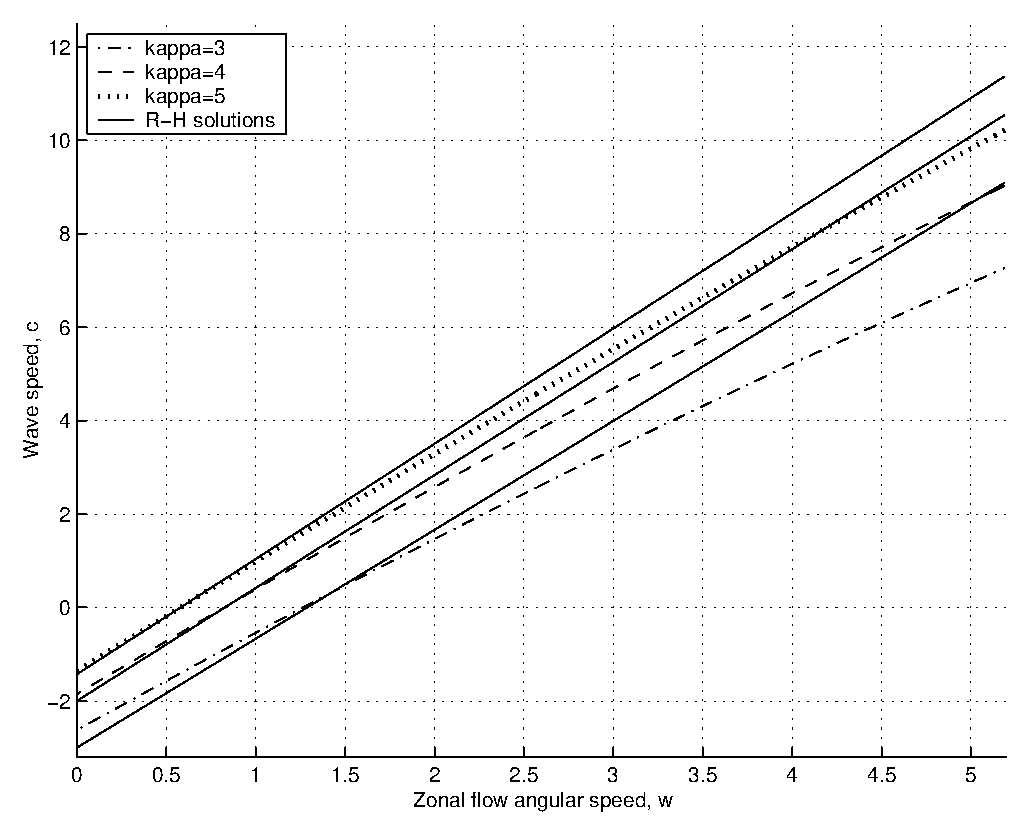
\includegraphics[scale=0.7]{IMAGES/wvchconstcomp.eps}
	\caption{Comparison of compressible linearized and Rossby--Haurwitz solutions for $\kappa=3,4$ and 5 with $N=100$.}
	\label{fig:wvccomp}
\end{figure}
To \index{Rossby--Haurwitz!comparison with compressible\\linearized solution}compare the two solution types we consider the primary physical eigenvalues for $\kappa=3,4$ and 5 with the equivalent Rossby--Haurwitz solutions over a reasonable range of allowable $\omega$ values. Figure~\ref{fig:wvccomp} shows the results of this comparison, with the solid lines representing the equivalent Rossby--Haurwitz solution for $\kappa=3$ to 5 from bottom to top respectively. In general one can conclude that the two models are in good broad agreement and we see that the behaviour of the compressible linearized solutions in not dissimilar to that of the incompressible linearized solutions, as shown in Figure~\ref{fig:wvcincomp} of Chapter~\ref{chap:2}. We also note that because the Haurwitz model has no provision for fixing the total mass $M_b$ of the atmosphere, differences are to be expected between that model and the work presented here. The discrepancies are most noticeable for larger values of the parameter $\omega$ where the effect of the mass matching condition has greater influence on the solution.

Figures~\ref{fig:swfscontscomp}--\ref{fig:swpcontscomp} present \index{polar stereographic projection}polar stereographic projections of the free-surface, density and pressure contours respectively. The scaling of the amplitude, via the linearization parameter $\epsilon$, was chosen so that the free-surface \index{height field matching}height matched the non-dimensional height of the Rossby--Haurwitz wave at $(\eta,\phi)=(0,\pi/4)$. This is similar to the technique that was used to match the incompressible and Rossby--Haurwitz solutions in Section~\ref{subsec:rhandlincomp} of Chapter~\ref{chap:2}. The scaling is arbitrary and is only used here so that visual confirmation of the general wave structure can be made.

\begin{figure}[htbp]
	\centering
		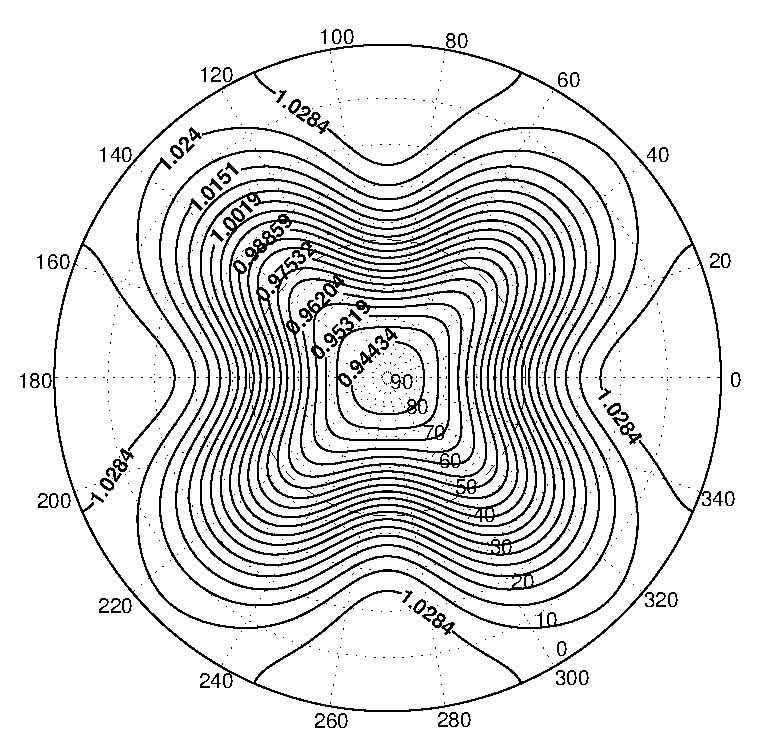
\includegraphics[scale=0.75]{IMAGES/swfscontscomp.eps}
	\caption{Compressible linearized free-surface contours for $\kappa=4$ with $N=100$.}
	\label{fig:swfscontscomp}
\end{figure}
It is evident that the compressible free-surface contours of Figure~\ref{fig:swfscontscomp} are quite similar in shape to those of the incompressible linearized theory (see Figure~\ref{fig:swfsconts}) and hence need no further comment. The density and pressure contours can be constructed once the free-surface shape is given, according to \eqref{eq:dencompnon2} and \eqref{eq:pcompnon2}. Examination of the density contours in Figure~\ref{fig:swrhocontscomp} reveals that the fluctuation in density about the mean sea-level value of $\rho=1$ is in reasonable agreement with that normally encountered in the Earth's atmosphere. Density values in Figure~\ref{fig:swrhocontscomp} range from approximately 85\% to 110\% of the mean sea-level value. Similar fluctuations are observed in the pressure field of Figure~\ref{fig:swpcontscomp}. Note also that the pressure and density contours are nearly parallel, so that the flow can be described as departing only slightly from that of \index{barotropic flow}barotropic flow.
\begin{figure}[htbp]
	\centering
		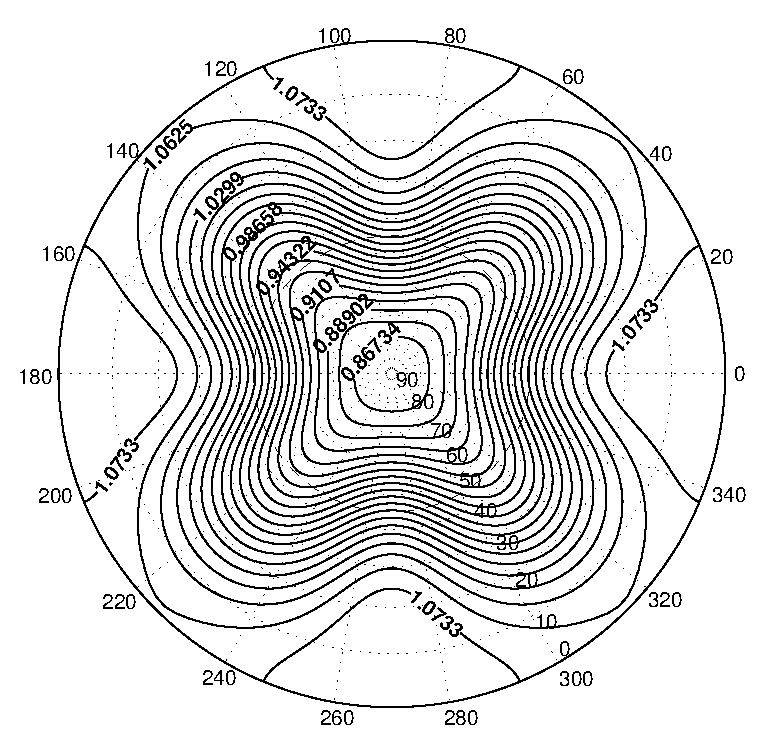
\includegraphics[scale=0.80]{IMAGES/swrhocontscomp.eps}
	\caption{Compressible linearized density contours for $\kappa=4$ with $N=100$.}
	\label{fig:swrhocontscomp}
\end{figure}

\begin{figure}[htbp]
	\centering
		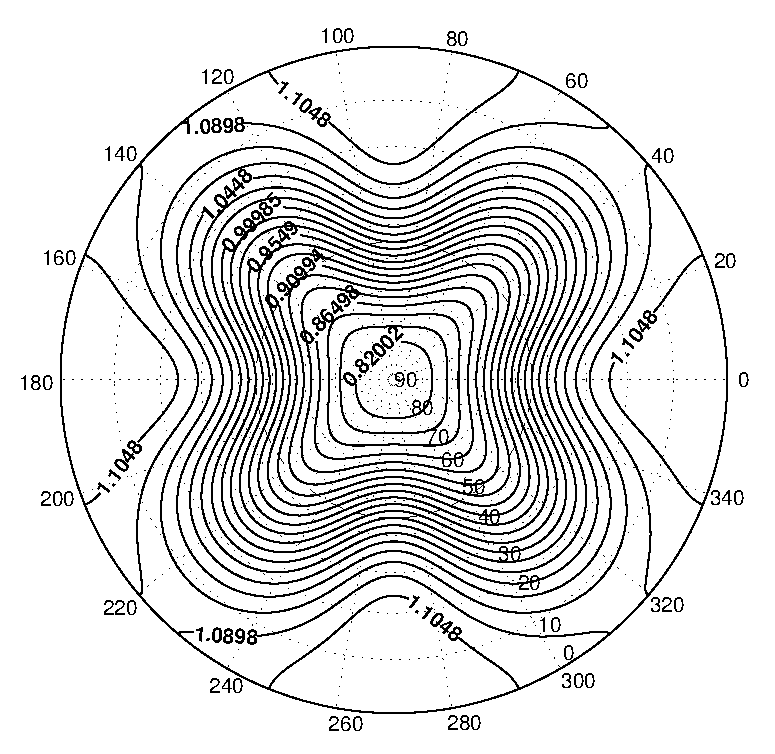
\includegraphics[scale=0.75]{IMAGES/swpcontscomp.eps}
	\caption{Compressible linearized pressure contours for $\kappa=4$ with $N=100$.}
	\label{fig:swpcontscomp}
\end{figure}

\begin{figure}[htbp]
	\centering
		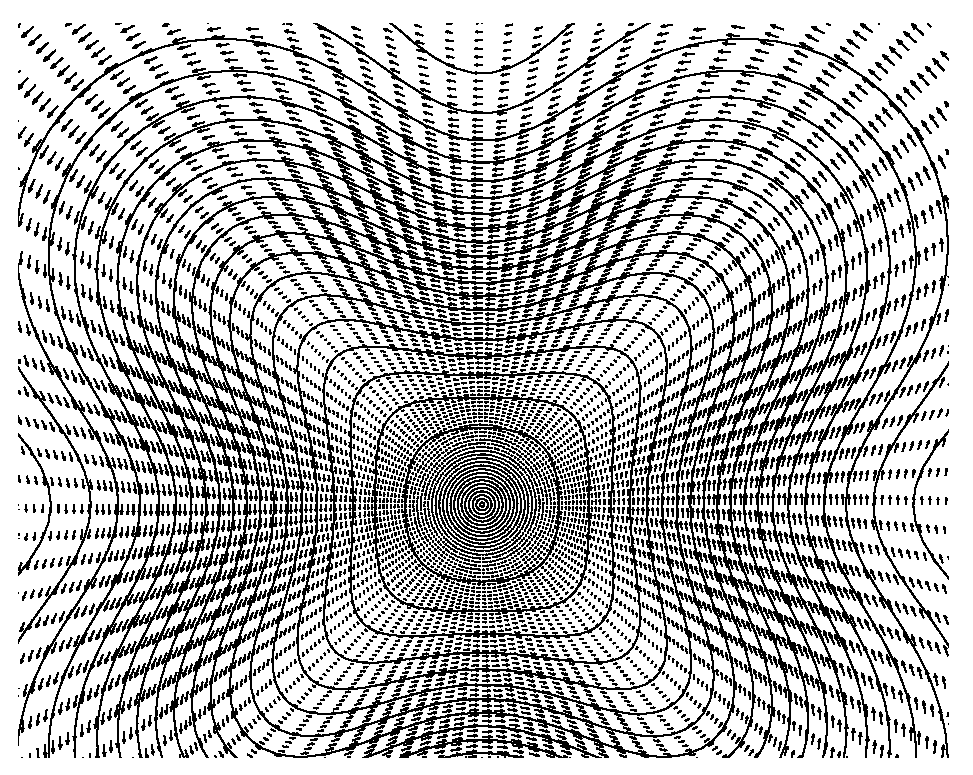
\includegraphics[scale=0.75]{IMAGES/pandvelfieldcomp.eps}
	\caption{Compressible linearized pressure contours with corresponding velocity vector field for $\kappa=4$ with $N=100$}
	\label{fig:pandvelfieldcomp}
\end{figure}

Figure~\ref{fig:pandvelfieldcomp} demonstrates the nature of the velocity vector field associated with the pressure field of Figure~\ref{fig:swpcontscomp}. The flow is observed to be predominantly \index{geostrophic approximation}geostrophic with the fluid streamlines essentially coinciding with the pressure contours.  Additionally we have increasingly diminishing flow as we approach either pole, which converges to the required stagnation point when $\phi=\pm \pi/2$.  The general nature of the fluid flow is directed in the same direction as the underlying zonal flow with the Rossby wave pattern moving relative to this mean fluid progression in an anti-clockwise manner, as expected for this particular map projection of the Northern Hemisphere.
